\chapter{TỔNG QUAN NGHIÊN CỨU VÀ CƠ SỞ LÝ LUẬN}

Chương này trình bày bối cảnh và động lực nghiên cứu, hệ thống hóa cơ sở lý thuyết về tín dụng, rủi ro và phân loại nhóm nợ, giới thiệu các mô hình học máy được luận văn sử dụng, đồng thời tổng quan các nghiên cứu liên quan để xác định khoảng trống nghiên cứu và định hướng của luận văn.

\section{Bối cảnh và động lực nghiên cứu}

\subsection{Hoạt động tín dụng và rủi ro tín dụng}

Hoạt động tín dụng có vai trò đặc biệt quan trọng đối với ngân hàng thương mại: đây là kênh cung ứng vốn chính cho cá nhân và tổ chức, đồng thời tạo nguồn thu từ lãi và phí. Do nghĩa vụ trả nợ được thực hiện trong tương lai, ngân hàng luôn đối mặt với sự không chắc chắn về khả năng trả nợ của khách hàng — tức rủi ro tín dụng, phát sinh khi khách hàng hoặc đối tác không thực hiện đầy đủ nghĩa vụ tài chính theo cam kết. Rủi ro này có thể bắt nguồn từ năng lực tài chính suy giảm, dòng tiền không ổn định, quản trị doanh nghiệp yếu, biến động thu nhập hoặc môi trường kinh doanh, thông tin không đầy đủ hoặc hành vi gian lận; hậu quả có thể thể hiện qua nợ quá hạn, nợ xấu, chi phí dự phòng tăng và mức độ an toàn vốn suy giảm.

Trong quản trị hiện đại, đánh giá tín dụng không nên chỉ được thực hiện một lần tại thời điểm phê duyệt, mà cần được cập nhật trong toàn bộ vòng đời khoản vay — theo dõi sự thay đổi của dư nợ, hành vi thanh toán, thời hạn, tình trạng cơ cấu lại và nhóm nợ. Điều này tạo ra nhu cầu xây dựng các mô hình có khả năng học từ dữ liệu lịch sử và hỗ trợ dự báo rủi ro theo thời gian.

\subsection{Chuyển đổi số trong ngân hàng và vai trò của dữ liệu}

Chuyển đổi số trong ngân hàng không chỉ là số hóa kênh giao dịch mà còn bao gồm tái cấu trúc quy trình nghiệp vụ, tự động hóa vận hành, xây dựng nền tảng dữ liệu và ứng dụng các mô hình phân tích trong quản trị. Trong tín dụng, ngân hàng có thể khai thác nhiều nhóm dữ liệu như thông tin định danh, lịch sử hợp đồng, dư nợ, hạn mức, số ngày quá hạn, thời hạn khoản vay, mục đích vay, nhóm nợ, trạng thái cơ cấu lại và dữ liệu hành vi. Khi dữ liệu được làm sạch và quản trị phù hợp, các mô hình học máy có thể hỗ trợ nhận diện quy luật mà quy tắc thủ công khó phát hiện; tuy nhiên, dữ liệu ngân hàng cũng có những thách thức như giá trị thiếu, sai lệch nghiệp vụ, mất cân bằng lớp, thay đổi theo thời gian và nguy cơ rò rỉ thông tin.

\subsection{Giới hạn của thông tin CIC và yêu cầu về công cụ cảnh báo sớm nội bộ}
\label{sec:cic-limits}

Thông tin nhóm nợ tại thời điểm báo cáo mô tả trạng thái đã được ghi nhận của khách hàng hoặc khoản vay. Việc dùng các trường trực tiếp hình thành nhóm nợ, chẳng hạn số ngày quá hạn, để phân loại lại chính trạng thái đó có thể tạo ra kết quả cao nhưng chưa chứng minh được khả năng dự báo diễn biến tiếp theo. Trong luận văn, bài toán phân loại hiện tại được dùng để đối sánh mô hình; bài toán chuyển nhóm được xây dựng riêng để khảo sát tín hiệu cảnh báo sớm.

Việc tổ chức tín dụng sử dụng thông tin CIC và hệ thống xếp hạng tín dụng nội bộ cần được đặt trong khuôn khổ quy định về phân loại tài sản có. Thông tư số 31/2024/TT-NHNN, có hiệu lực từ ngày 01/07/2024 và thay thế Thông tư số 11/2021/TT-NHNN, đã được sửa đổi, bổ sung bởi Thông tư số 37/2025/TT-NHNN \cite{sbv2024tt31,sbv2025tt37}. Luận văn sử dụng các văn bản này làm căn cứ về bối cảnh phân loại nợ; kết quả của mô hình nghiên cứu chưa phải căn cứ để thay thế quy trình phân loại nợ theo quy định.

Công cụ cảnh báo sớm nội bộ có thể hỗ trợ lựa chọn hồ sơ cần rà soát dựa trên thông tin sẵn có tại thời điểm đánh giá. Nghiên cứu hiện tại chưa đo lường độ trễ cập nhật, chi phí tra cứu hoặc hiệu quả của quy trình sử dụng CIC, nên không thực hiện đối sánh hiệu quả với CIC. Mục~\ref{sec:scope-transition} (Chương 2) cụ thể hóa bài toán dự báo chuyển nhóm trong phạm vi dữ liệu cho phép.

\section{Nền tảng tín dụng, rủi ro và phân loại nhóm nợ}

\subsection{Khái niệm tín dụng và rủi ro tín dụng}

Tín dụng là quan hệ kinh tế trong đó bên cho vay chuyển giao quyền sử dụng một lượng giá trị cho bên đi vay trong một khoảng thời gian xác định, với nghĩa vụ hoàn trả theo các điều kiện đã thỏa thuận.

Rủi ro tín dụng là khả năng phát sinh tổn thất do khách hàng hoặc đối tác không thực hiện đầy đủ nghĩa vụ tài chính. Rủi ro chịu ảnh hưởng từ năng lực tài chính, đặc điểm khoản vay, lịch sử tín dụng, chính sách cấp tín dụng và điều kiện kinh tế.

\subsection{Phân loại nhóm nợ}

\begin{table}[H]
\centering
\caption{Các nhóm nợ trong nghiên cứu}
\begin{tabular}{|c|p{4cm}|p{7cm}|}
\hline
1 & Nợ đủ tiêu chuẩn & Mức rủi ro thấp.\\
\hline
2 & Nợ cần chú ý & Đã xuất hiện dấu hiệu cần theo dõi.\\
\hline
3 & Nợ dưới tiêu chuẩn & Khả năng thu hồi suy giảm đáng kể.\\
\hline
4 & Nợ nghi ngờ & Mức rủi ro cao.\\
\hline
5 & Nợ có khả năng mất vốn & Mức rủi ro cao nhất.\\
\hline
\end{tabular}
\end{table}

\subsection{Xếp hạng tín dụng và tổn thất kỳ vọng}

Xếp hạng tín dụng là quá trình gán khách hàng hoặc khoản vay vào một hạng rủi ro dựa trên thông tin tài chính, đặc điểm khoản vay và lịch sử thực hiện nghĩa vụ. Trong phạm vi luận văn, năm nhóm nợ được xem là các mức rủi ro có thứ tự; mô hình được xây dựng để hỗ trợ nhận diện nhóm nợ tương ứng của từng quan sát.

Tổn thất kỳ vọng có thể biểu diễn:
\[
EL=PD\times LGD\times EAD.
\]
Trong đó $EL$ là tổn thất kỳ vọng; $PD$ là xác suất vỡ nợ trong kỳ đánh giá; $LGD$ là tỷ lệ tổn thất khi vỡ nợ sau khi xét khả năng thu hồi; và $EAD$ là dư nợ tại thời điểm vỡ nợ. Luận văn hiện tập trung vào phân loại trạng thái rủi ro, chưa trực tiếp ước lượng đủ ba cấu phần của $EL$ \cite{basel_framework}.

\begin{figure}[H]
\centering
\begin{tikzpicture}[
    >=stealth,
    font=\small,
    riskbox/.style={draw, rounded corners=2pt, align=center, minimum height=1.8cm, text width=3.7cm},
    resultbox/.style={draw, rounded corners=2pt, very thick, align=center, minimum height=1.45cm, text width=4.2cm}
]
    \node[riskbox] (pd) at (-5.0,1.6)
        {\textbf{$PD$}\\Xác suất khách hàng vỡ nợ trong kỳ đánh giá};
    \node[riskbox] (lgd) at (0,1.6)
        {\textbf{$LGD$}\\Tỷ lệ tổn thất sau khi xét phần có thể thu hồi};
    \node[riskbox] (ead) at (5.0,1.6)
        {\textbf{$EAD$}\\Dư nợ của khoản cấp tín dụng tại thời điểm vỡ nợ};
    \node[resultbox] (el) at (0,-1.25)
        {\textbf{Tổn thất kỳ vọng}\\$EL=PD\times LGD\times EAD$};
    \draw[->, very thick] (pd.south) -- (el.north west);
    \draw[->, very thick] (lgd.south) -- (el.north);
    \draw[->, very thick] (ead.south) -- (el.north east);
\end{tikzpicture}
\caption{Các cấu phần của tổn thất kỳ vọng trong rủi ro tín dụng}
\label{fig:el-components}
\caption*{\textit{Nguồn: Tác giả tổng hợp và vẽ lại từ Basel Committee on Banking Supervision \cite{basel_framework}.}}
\end{figure}

\section{Sự phát triển của các phương pháp đánh giá tín dụng và tổng quan nghiên cứu liên quan}
\label{sec:ch1-history}

Đánh giá tín dụng đã trải qua ba giai đoạn phát triển chính. Giai đoạn đầu dựa trên phương pháp chuyên gia, tiêu biểu là khung 5C (\textit{Character, Capacity, Capital, Collateral, Conditions}) — công cụ tổ chức thông tin để cán bộ tín dụng tổng hợp nhận định, không phải thuật toán tự động tạo xác suất vỡ nợ \cite{hand1997statistical,thomas2000survey}. Giai đoạn thứ hai chuyển sang các mô hình thống kê định lượng, mở đầu bằng phân tích phân biệt đa biến của Altman \cite{altman1968financial} và hồi quy logistic của Ohlson \cite{ohlson1980financial}, cho phép ước lượng xác suất rủi ro thay vì chỉ xếp loại theo kinh nghiệm, nhưng vẫn giả định quan hệ tuyến tính giữa biến đầu vào và rủi ro. Giai đoạn thứ ba là sự chuyển dịch sang các mô hình học máy, có khả năng nắm bắt quan hệ phi tuyến phức tạp hơn mà không cần thiết kế tương tác thủ công.

Các nghiên cứu tổng quan của Hand và Henley \cite{hand1997statistical}, Thomas \cite{thomas2000survey}, Crook \cite{crook2007recent} và các nghiên cứu đối chiếu mô hình của Baesens và cộng sự \cite{baesens2003benchmarking}, Lessmann và cộng sự \cite{lessmann2015benchmarking} hệ thống hóa quá trình chuyển dịch này, đồng thời mở rộng phạm vi đánh giá từ thời điểm phê duyệt sang theo dõi hành vi trong vòng đời khoản vay. Điểm chung được các tác giả nhấn mạnh là không tồn tại một thuật toán luôn vượt trội trên mọi bộ dữ liệu; hiệu quả phụ thuộc vào chất lượng dữ liệu, cách chia mẫu và tiêu chí đánh giá được sử dụng.

\subsection{Tổng quan các nghiên cứu liên quan}

Brown và Mues \cite{brown2012experimental} nhấn mạnh ảnh hưởng của mất cân bằng lớp đến hiệu năng mô hình. Xia và cộng sự \cite{xia2017boosted} cho thấy boosted tree có khả năng cải thiện dự báo. Barboza và cộng sự \cite{barboza2017machine} ghi nhận kết quả cạnh tranh của các mô hình cây trong dự báo phá sản. Dastile và cộng sự \cite{dastile2020statistical} chỉ ra các hạn chế phổ biến về dữ liệu nhỏ, mất cân bằng, thiếu chuẩn đánh giá và khả năng giải thích.

Tại Việt Nam, nghiên cứu thường tập trung vào đánh giá rủi ro tín dụng cá nhân, rủi ro doanh nghiệp và dự báo nợ xấu; tuy nhiên chưa có nhiều nghiên cứu công bố việc phân loại trực tiếp năm nhóm nợ trên dữ liệu thực tế, kết hợp so sánh nhiều mô hình, chia dữ liệu theo thời gian, đánh giá có xét thứ tự và phân tích khả năng giải thích.

\subsection{Khoảng trống nghiên cứu và định vị đề tài}
\label{sec:ch1-gaps}

Từ bối cảnh và tổng quan nghiên cứu trên, có thể xác định ba khoảng trống liên quan trực tiếp đến nghiên cứu của luận văn:
\begin{enumerate}
    \item \textit{Về đối tượng bài toán và nguồn dữ liệu.} Phần lớn nghiên cứu ứng dụng học máy trong tín dụng đặt mục tiêu nhị phân (tốt/xấu) hoặc dự báo phá sản doanh nghiệp, chủ yếu trên các bộ dữ liệu công khai có quy mô nhỏ và thời gian thu thập đã cũ. Bài toán phân loại năm nhóm nợ có thứ tự theo quy định phân loại nợ tại Việt Nam ít được khảo sát trực tiếp trên dữ liệu thực tế của ngân hàng thương mại trong nước, vốn hiếm khi được công bố hoặc sử dụng trong nghiên cứu học thuật.
    \item \textit{Về khả năng cảnh báo sớm.} Thông tin nhóm nợ từ CIC mang tính hồi cứu (Mục~\ref{sec:cic-limits}), trong khi Thông tư số 31/2024/TT-NHNN (thay thế Thông tư số 11/2021/TT-NHNN) yêu cầu tổ chức tín dụng xây dựng hệ thống xếp hạng tín dụng nội bộ \cite{sbv2024tt31,sbv2025tt37}. Tuy vậy, khả năng dự báo một khoản vay chuyển sang nhóm nợ cao hơn trong ngắn hạn bằng học máy, tức cơ sở của công cụ cảnh báo sớm nội bộ, chưa được kiểm chứng bằng thực nghiệm trên dữ liệu ngân hàng Việt Nam.
    \item \textit{Về phương pháp và thiết kế đánh giá.} Tính thứ tự của năm nhóm nợ chưa được khai thác trong thiết kế đánh giá của phần lớn nghiên cứu tham khảo; phép chia mẫu ngẫu nhiên vẫn phổ biến hơn chia mẫu theo thời gian dù rủi ro tín dụng mang tính thời điểm; và các mô hình boosting thường thiếu khả năng giải thích đi kèm.
\end{enumerate}

Luận văn định vị đóng góp vào khoảng trống (1) và (2). Toàn bộ thực nghiệm được thực hiện trên hai bộ dữ liệu thực tế của cùng một ngân hàng thương mại Việt Nam, với bài toán phân loại năm nhóm nợ theo đúng quy định phân loại nợ trong nước; song song đó, luận văn xây dựng và đánh giá trung thực bài toán dự báo chuyển nhóm nợ trong ngắn hạn nhằm trả lời trực tiếp yêu cầu về công cụ cảnh báo sớm. Với khoảng trống (3), luận văn xử lý mất cân bằng lớp theo cả hai hướng lý thuyết (Mục~\ref{sec:imbalance-theory}) và giải thích mô hình bằng SHAP, nhưng chưa lượng hóa sai số theo thứ tự nhóm nợ trong các bảng kết quả chính.

Trên cơ sở các khoảng trống trên, đóng góp của luận văn thể hiện ở thiết kế bài toán và tổ chức thực nghiệm trên dữ liệu tín dụng thực tế:
\begin{enumerate}
    \item đối sánh mô hình phân loại năm nhóm nợ trên hai cấu trúc dữ liệu của cùng một ngân hàng, kết hợp đối chiếu bốn chiến lược xử lý mất cân bằng lớp (không xử lý, trọng số lớp, SMOTE, kết hợp), với năm mô hình trong bảng kết quả chính của bộ A và sáu mô hình của bộ B;
    \item đánh giá vai trò của số lượng đặc trưng và các nhóm thông tin nghiệp vụ đối với hiệu quả phân loại; đối chiếu mức độ quan trọng bằng SHAP trên cả hai bộ dữ liệu độc lập để kiểm tra tính nhất quán của kết luận;
    \item xây dựng và đánh giá trung thực bài toán dự báo chuyển nhóm nợ trong ngắn hạn trên hai cặp kỳ báo cáo thật liên tiếp của bộ B, bao gồm cả kiểm tra độ ổn định của kết quả giữa hai cặp kỳ độc lập, thay vì chỉ báo cáo kết quả của một cặp kỳ duy nhất.
\end{enumerate}
Luận văn không đề xuất thuật toán mới; đóng góp nằm ở thiết kế bài toán và cách tổ chức, kiểm chứng thực nghiệm trên dữ liệu tín dụng thực tế.

\section{Từ đánh giá truyền thống đến các mô hình học máy}
\label{sec:ch2-models}

Học máy là nhánh của trí tuệ nhân tạo trong đó mô hình học quy luật từ dữ liệu thay vì được lập trình theo quy tắc cố định; bài toán của luận văn thuộc học có giám sát. So với phương pháp chuyên gia (khai thác được thông tin định tính nhưng chủ quan) và các mô hình thống kê tuyến tính như Z-score của Altman hay Logistic Regression (dễ giải thích nhưng khó tự động nắm bắt tương tác phức tạp), các mô hình học máy dưới đây được lựa chọn nhằm mở rộng khả năng nắm bắt quan hệ phi tuyến.

\subsection{Mô hình tuyến tính và cây quyết định}

\noindent\textbf{Logistic Regression đa lớp.}

\[
P(Y=k\mid\mathbf{x})
=
\frac{\exp(\beta_{k0}+\boldsymbol{\beta}_{k}^{T}\mathbf{x})}
{\sum_{j=1}^{K}\exp(\beta_{j0}+\boldsymbol{\beta}_{j}^{T}\mathbf{x})}.
\]
Trong đó $K$ là số lớp; $\mathbf{x}$ là véc-tơ đặc trưng; $\beta_{k0}$ là hệ số chặn của lớp $k$; $\boldsymbol{\beta}_{k}$ là véc-tơ hệ số của lớp $k$; và mẫu số chuẩn hóa để tổng xác suất của $K$ lớp bằng 1 \cite{hosmer2013applied}.

\medskip
\noindent\textbf{Decision Tree.}

Decision Tree chia không gian đặc trưng bằng các điều kiện dạng $x_j\le s$. Mô hình dễ diễn giải nhưng có thể quá khớp nếu không kiểm soát độ sâu và số quan sát tại lá.

\medskip
\noindent\textbf{Random Forest.}

\[
\hat{y}=\operatorname{mode}\{h_b(\mathbf{x})\}_{b=1}^{B}.
\]
Trong đó $B$ là số cây; $h_b(\mathbf{x})$ là dự báo lớp của cây thứ $b$ tại hồ sơ $\mathbf{x}$; và $\operatorname{mode}$ chọn lớp xuất hiện nhiều nhất trong các dự báo cây \cite{breiman2001random}.

\subsection{Các mô hình boosting}

\noindent\textbf{XGBoost.}

\[
\mathcal{L}^{(t)}
=
\sum_{i=1}^{n}
l(y_i,\hat{y}_{i}^{(t-1)}+f_t(\mathbf{x}_i))
+\Omega(f_t).
\]
Trong đó $t$ là vòng boosting; $n$ là số quan sát huấn luyện; $l(\cdot)$ là hàm mất mát; $\hat{y}_{i}^{(t-1)}$ là dự báo tích lũy trước vòng $t$; $f_t$ là cây mới; và $\Omega(f_t)$ là số hạng phạt độ phức tạp của cây nhằm hạn chế quá khớp \cite{chen2016xgboost}.

\begin{figure}[H]
\centering
\begin{minipage}{0.46\textwidth}
    \centering
    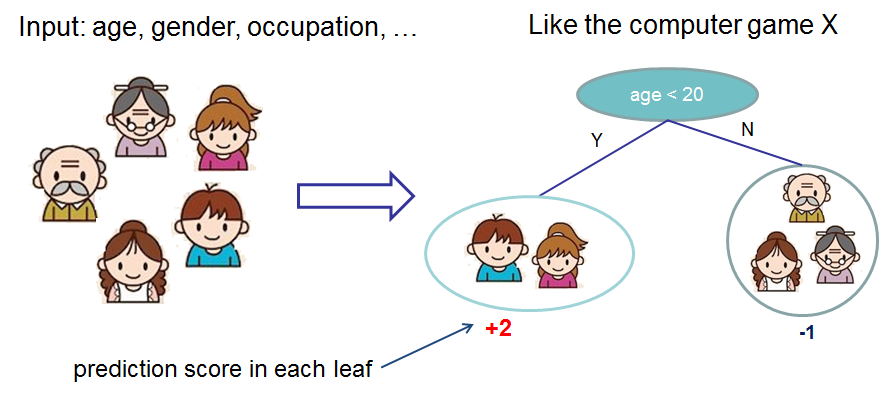
\includegraphics[width=\linewidth]{figures/xgboost_cart_example.png}
    \\[1mm]\small (a) Một cây CART đơn — mỗi hồ sơ nhận điểm dự báo tại lá tương ứng
\end{minipage}
\hfill
\begin{minipage}{0.5\textwidth}
    \centering
    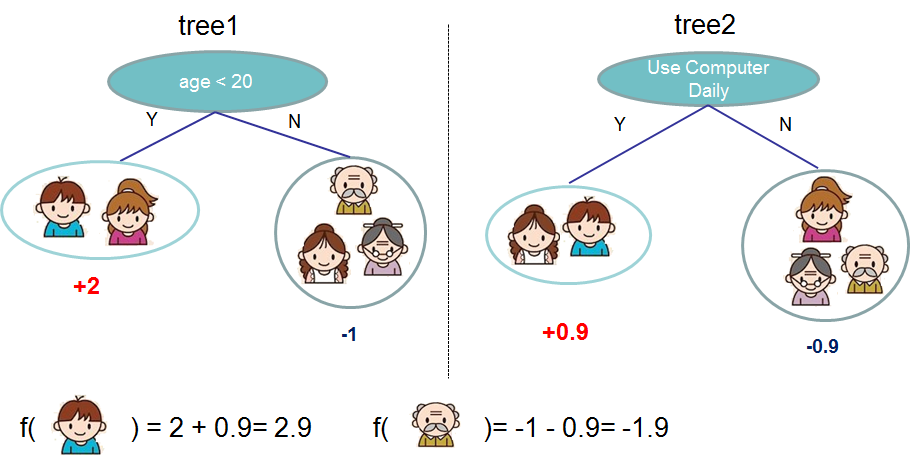
\includegraphics[width=\linewidth]{figures/xgboost_two_trees.png}
    \\[1mm]\small (b) Cộng dồn điểm dự báo của nhiều cây: $f(\mathbf{x})=\sum_t f_t(\mathbf{x})$
\end{minipage}
\caption{Cơ chế cộng dồn các cây trong XGBoost}
\label{fig:xgboost-additive}
\caption*{\textit{Nguồn: Tài liệu chính thức của XGBoost \cite{xgboost_docs}, giấy phép Apache 2.0; minh họa cho cơ chế mô tả trong Chen và Guestrin \cite{chen2016xgboost}; truy cập ngày 15/08/2026.}}
\end{figure}

Hình~\ref{fig:xgboost-additive} thể hiện cách dự báo được cập nhật tuần tự. Mỗi cây mới $f_t(\mathbf{x})$ hiệu chỉnh phần sai số còn lại của tổ hợp trước đó bằng cách cộng thêm điểm số tại lá tương ứng của hồ sơ đang xét, có nhân hệ số học $\eta$; XGBoost đồng thời đưa số hạng chính quy $\Omega(f_t)$ vào hàm mục tiêu để kiểm soát độ phức tạp.

\medskip
\noindent\textbf{LightGBM.}

LightGBM tối ưu tốc độ và bộ nhớ bằng các kỹ thuật như Gradient-based One-Side Sampling và Exclusive Feature Bundling. Thuật toán phát triển cây theo lá tốt nhất, tức là tại mỗi bước ưu tiên tách lá tạo ra mức giảm hàm mất mát lớn nhất. Cách phát triển này có thể hội tụ nhanh nhưng cũng làm cây mất cân đối và dễ quá khớp khi dữ liệu nhỏ; vì vậy cần kiểm soát \mbox{\texttt{num\_leaves}}, \mbox{\texttt{min\_data\_in\_leaf}} và \mbox{\texttt{max\_depth}} \cite{ke2017lightgbm,lightgbm_docs}.

\begin{figure}[H]
\centering
\begin{minipage}{0.48\textwidth}
    \centering
    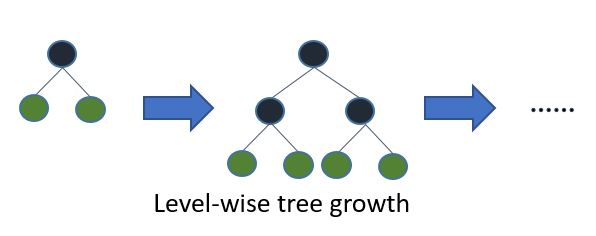
\includegraphics[width=\linewidth]{figures/lightgbm_level_wise.png}
    \\[1mm]\small (a) Phát triển cây theo tầng
\end{minipage}
\hfill
\begin{minipage}{0.48\textwidth}
    \centering
    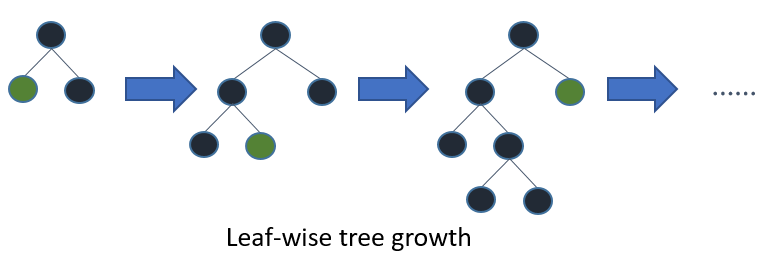
\includegraphics[width=\linewidth]{figures/lightgbm_leaf_wise.png}
    \\[1mm]\small (b) Phát triển cây theo lá tốt nhất
\end{minipage}
\caption{Minh họa hai chiến lược phát triển cây quyết định}
\label{fig:lightgbm-official-growth}
\caption*{\textit{Nguồn: Tài liệu chính thức của LightGBM \cite{lightgbm_docs}, giấy phép MIT; truy cập ngày 15/08/2026.}}
\end{figure}

Hình \ref{fig:lightgbm-official-growth} cho thấy sự khác biệt trực quan giữa hai chiến lược. Phương pháp theo tầng mở rộng đồng thời các nút ở cùng độ sâu và thường tạo ra cấu trúc tương đối cân đối. Ngược lại, LightGBM tiếp tục phân chia lá mang lại mức giảm hàm mất mát lớn nhất, vì vậy cây có thể phát triển không đối xứng. Cơ chế này góp phần nâng cao hiệu quả tối ưu, nhưng đồng thời đòi hỏi kiểm soát độ sâu và số lá để hạn chế hiện tượng quá khớp \cite{ke2017lightgbm,lightgbm_docs}.

\medskip
\noindent\textbf{CatBoost.}

CatBoost có khả năng xử lý trực tiếp biến phân loại và sử dụng cơ chế \textit{ordered boosting} để hạn chế rò rỉ thông tin trong quá trình huấn luyện \cite{prokhorenkova2018catboost}.

\section{Những thách thức khi mô hình hóa dữ liệu tín dụng}

\subsection{Thách thức đối với hiệu năng dự báo}

\noindent\textbf{Mất cân bằng lớp.}
\label{sec:imbalance-theory}

Khi các nhóm nợ có tần suất chênh lệch lớn, mô hình có xu hướng thiên về lớp đa số. Hai hướng xử lý phổ biến, độc lập nhau và có thể kết hợp, là điều chỉnh ở cấp thuật toán (trọng số lớp trong hàm mất mát) và điều chỉnh ở cấp dữ liệu (sinh thêm quan sát tổng hợp cho lớp thiểu số).

\noindent\textit{Cấp thuật toán — trọng số lớp.}
\[
\mathcal{L}
=
-\sum_{i=1}^{N}
w_{y_i}
\sum_{k=1}^{K}
\mathbb{I}(y_i=k)\log p_{ik}.
\]
Trong đó $N$ là số quan sát; $K$ là số lớp; $w_{y_i}$ là trọng số gán cho lớp thật của quan sát $i$; $\mathbb{I}(y_i=k)$ bằng 1 khi $y_i=k$ và bằng 0 trong trường hợp khác; $p_{ik}$ là xác suất dự báo lớp $k$. Trọng số lớn hơn cho lớp hiếm làm sai số của lớp đó có ảnh hưởng lớn hơn tới hàm mất mát. Trọng số thường được tính theo tần suất nghịch đảo:
\[
w_c=\frac{N}{K\,n_c},
\]
trong đó $n_c$ là số quan sát thuộc lớp $c$; mỗi quan sát $i$ được gán trọng số $w_{y_i}$.

\noindent\textit{Cấp dữ liệu — SMOTE.} SMOTE (\textit{Synthetic Minority Over-sampling Technique}) tạo một điểm tổng hợp cho lớp thiểu số bằng nội suy tuyến tính giữa một quan sát và một láng giềng gần cùng lớp:
\[
\mathbf{x}_{\mathrm{new}}
=
\mathbf{x}_i+\lambda\left(\mathbf{x}_{nn}-\mathbf{x}_i\right),
\qquad \lambda\sim U(0,1),
\]
trong đó $\mathbf{x}_i$ là véc-tơ của một quan sát lớp thiểu số; $\mathbf{x}_{nn}$ là một trong các láng giềng gần của nó; $\lambda$ là số ngẫu nhiên phân bố đều trên $[0,1]$; và $\mathbf{x}_{\mathrm{new}}$ là điểm nội suy \cite{chawla2002smote}. Khác với trọng số lớp (không đổi số quan sát, chỉ đổi ảnh hưởng của từng quan sát lên hàm mất mát), SMOTE làm tăng số quan sát huấn luyện của lớp thiểu số bằng dữ liệu nội suy chứ không phải quan sát độc lập mới. Hai hướng có thể dùng riêng hoặc kết hợp; hiệu quả thực tế của từng chiến lược trên dữ liệu của luận văn được đối chiếu thực nghiệm ở Mục~\ref{sec:imbalance} (Chương 2) và Mục~\ref{sec:imbalance-combined-results} (Chương 3).

\medskip
\noindent\textbf{Tính thứ tự.}
Năm nhóm nợ có thứ tự rủi ro từ thấp đến cao nên hai sai số lệch một bậc và lệch bốn bậc không có mức độ nghiêm trọng như nhau. Ordinal MAE, trình bày tại Mục~\ref{sec:metrics} (Chương 3), là một thước đo có thể bổ sung để lượng hóa số bậc sai lệch trung bình. Các bảng thực nghiệm hiện tại chưa báo cáo chỉ tiêu này, nên kết luận về mô hình chưa bao gồm đánh giá định lượng theo thứ tự nhóm nợ.

\subsection{Khả năng giải thích và yêu cầu ứng dụng}
\label{sec:shap-theory}

\[
f(\mathbf{x})=\phi_0+\sum_{j=1}^{p}\phi_j.
\]
Trong đó $f(\mathbf{x})$ là đầu ra mô hình cần giải thích; $\phi_0$ là giá trị nền; $p$ là số đặc trưng; và $\phi_j$ là đóng góp SHAP của đặc trưng $j$ cho hồ sơ $\mathbf{x}$ \cite{lundberg2017unified}.

\begin{figure}[H]
\centering
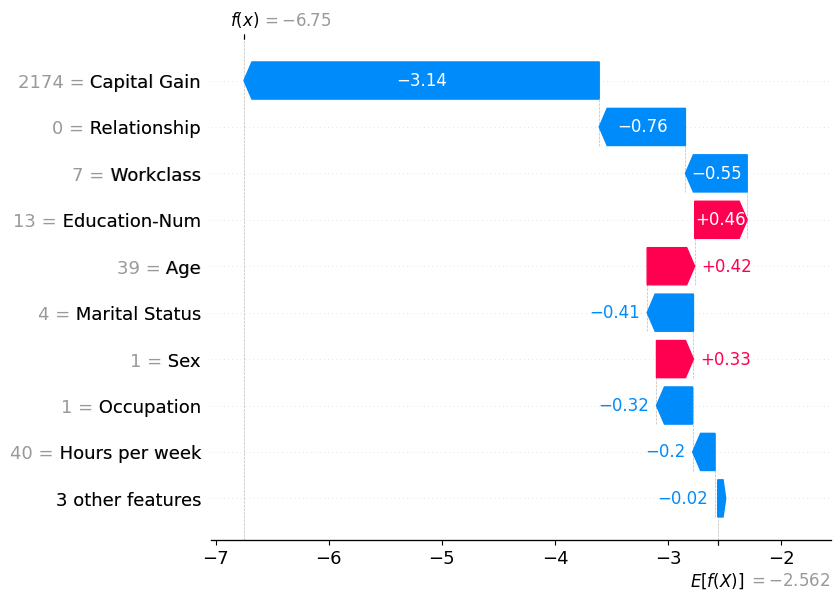
\includegraphics[width=0.72\textwidth]{figures/shap_waterfall_example.png}
\caption{Ví dụ biểu đồ waterfall minh họa nguyên lý phân rã dự báo theo giá trị SHAP}
\label{fig:shap-additive}
\caption*{\textit{Nguồn: Tài liệu chính thức của SHAP \cite{shap_docs}, giấy phép MIT, dựa trên phương pháp của Lundberg và Lee \cite{lundberg2017unified}; truy cập ngày 15/08/2026.}}
\end{figure}

Dự báo theo SHAP bắt đầu từ giá trị nền $\phi_0$ (ký hiệu $E[f(X)]$ trong Hình \ref{fig:shap-additive}), sau đó được điều chỉnh tăng hoặc giảm bởi đóng góp của từng đặc trưng cho tới khi đạt đầu ra $f(\mathbf{x})$ của hồ sơ đang xét. Dấu của $\phi_j$ cho biết chiều tác động đối với đầu ra đang được giải thích (thanh màu đỏ: đóng góp dương; thanh màu xanh: đóng góp âm), còn độ lớn tuyệt đối phản ánh cường độ đóng góp. Hình \ref{fig:shap-additive} chỉ minh họa nguyên lý phân rã từ tài liệu SHAP; các giá trị SHAP thực nghiệm của luận văn được tính riêng trên dữ liệu tín dụng ở Chương 3.

\begin{figure}[H]
\centering
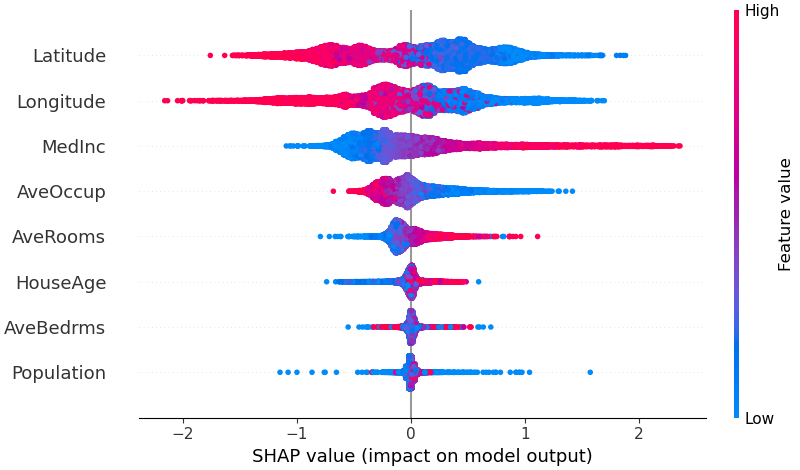
\includegraphics[width=0.82\textwidth]{figures/shap_beeswarm_example.png}
\caption{Ví dụ biểu đồ SHAP beeswarm trong phân tích mức độ tác động của đặc trưng}
\label{fig:shap-official-beeswarm}
\caption*{\textit{Nguồn: Kho tài liệu chính thức của SHAP \cite{shap_docs}, dựa trên phương pháp của Lundberg và Lee \cite{lundberg2017unified}, giấy phép MIT; truy cập ngày 15/08/2026.}}
\end{figure}

Trong biểu đồ beeswarm, mỗi điểm biểu thị một quan sát; vị trí trên trục hoành phản ánh giá trị SHAP, còn màu sắc thể hiện mức độ cao hoặc thấp của giá trị đặc trưng. Các đặc trưng được sắp xếp theo tổng độ lớn ảnh hưởng, qua đó cho phép xem xét đồng thời tầm quan trọng, chiều tác động và mức độ phân tán của ảnh hưởng trên toàn bộ tập dữ liệu. Hình \ref{fig:shap-official-beeswarm} chỉ minh họa cách đọc biểu đồ từ tài liệu SHAP; các kết luận thực nghiệm của luận văn được rút ra từ dữ liệu tín dụng và các biểu đồ được tạo riêng ở Chương 3.

\section{Tóm tắt chương}

Chương này đã trình bày bối cảnh và động lực nghiên cứu xuất phát từ vai trò của hoạt động tín dụng và rủi ro tín dụng trong ngân hàng thương mại, giới hạn hồi cứu của thông tin CIC và căn cứ pháp lý cho yêu cầu về công cụ cảnh báo sớm nội bộ (Mục~\ref{sec:cic-limits}); cơ sở lý thuyết về tín dụng, rủi ro và phân loại nhóm nợ; các mô hình học máy được sử dụng; những thách thức đặc thù của dữ liệu tín dụng; và tổng quan nghiên cứu liên quan làm cơ sở xác định ba khoảng trống nghiên cứu, định vị đề tài và đóng góp dự kiến của luận văn (Mục~\ref{sec:ch1-gaps}). Hệ thống chỉ tiêu đánh giá mô hình được trình bày cùng kết quả thực nghiệm tại Mục~\ref{sec:metrics} (Chương 3).

Trên cơ sở lý thuyết và định hướng đã xác lập, Chương 2 sẽ phát biểu hình thức hai bài toán nghiên cứu và trình bày cụ thể nguồn dữ liệu, quy trình xử lý, phân tích khám phá dữ liệu, xây dựng đặc trưng nghiệp vụ và phương pháp thực nghiệm được cài đặt trong mã nguồn trên hai bộ dữ liệu thực tế của luận văn.
